
%(BEGIN_QUESTION)
% Copyright 2009, Tony R. Kuphaldt, released under the Creative Commons Attribution License (v 1.0)
% This means you may do almost anything with this work of mine, so long as you give me proper credit

En reguleringsventil av spjeldtype skal brukes til å strupe forbrenningsluftstrømmen til en stor naturgassbrenner i en industriovn:

$$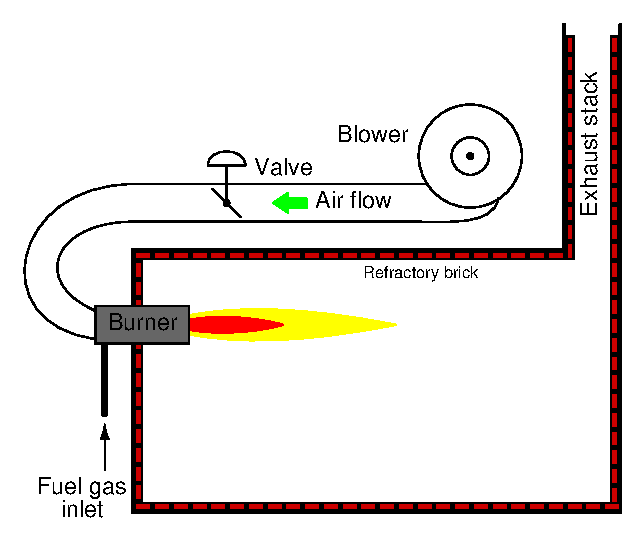
\includegraphics[width=15.5cm]{i01414x01.eps}$$

Trykkfallet over brenneren er 8 unser per kvadrattomme (8 oz/in$^{2}$). Ved ``high fire'' (full luftstrøm og full varmeeffekt fra brenneren) gir blåseren et statisk trykk på 35 "W.C. ved en strømningsrate på 2,000 standard kubikkfot per minutt (2,000 SCFM). Ovnstrykket reguleres til atmosfærisk trykk til enhver tid.

Gitt disse betingelsene: Hva må forbrenningsluft-ventilens $C_{v}$ være ved fullt åpen ventil for å slippe gjennom 2,000 SCFM til brenneren? Anta omgivelsestemperatur 45$^{o}$ F. Beregn også omtrentlig ventilstørrelse (nominell rørdiameter i tommer) som trengs dersom ventiltypen er et 90-graders spjeld med offset-sete ($C_d = 29$).

\vskip 10pt

Bruk følgende ventilkapasitetsligning i beregningene:

$$Q = 963 \> C_v \sqrt{{\Delta P (P_1 + P_2)} \over {G_g T}}$$

\noindent
Hvor,

$Q$ = Gasstrømningsrate, i enheten Standard Cubic Feet per Hour (SCFH)

$C_v$ = Ventilens kapasitetskoeffisient

$\Delta P$ = Trykkfall over ventilen, pounds per square inch differential (PSID)

$P_1$ = Oppstrøms ventiltrykk, pounds per square inch absolute (PSIA)

$P_2$ = Nedstrøms ventiltrykk, pounds per square inch absolute (PSIA)

$G_g$ = Gassens spesifikke vekt (luft ved standard temperatur og trykk = 1.0)

$T$ = Absolutt gasstemperatur i grader Rankine ($^{o}$R)


\vfil

\underbar{file i01414}
\eject
%(END_QUESTION)





%(BEGIN_ANSWER)

Dette er et gradert spørsmål -- ingen svar eller hint gis!

%(END_ANSWER)





%(BEGIN_NOTES)

Dette problemet er i praksis en ``sett inn og regn''-øvelse der vi løser for én variabel i en ligning ved å manipulere ligningen og sette inn alle kjente verdier for de andre variablene i riktige enheter. Først manipulerer vi strømningsligningen for å løse for $C_v$:

$$C_v = {Q \over 963 \sqrt{{\Delta P (P_1 + P_2)} \over {G_g T}}}$$

Deretter må vi bestemme verdiene til alle variabler (utenom $C_v$) for å kunne løse for $C_v$. Vi får oppgitt noen trykkverdier for systemet, men det kan være vanskelig å se nøyaktig hvordan de hører hjemme i ligningen ($\Delta P$, $P_1$, $P_2$). En nyttig problemløsningsmetode her er å sammenligne luftstrømrøret med en elektrisk krets, der blåseren representerer en spenningskilde, ventilen representerer en variabel motstand, og brenneren representerer en fast motstand. Siden blåseren suger luft fra atmosfæren og brenneren slipper luft ut til atmosfæren, vil disse punktene i analogien representeres som {\it jord}:

$$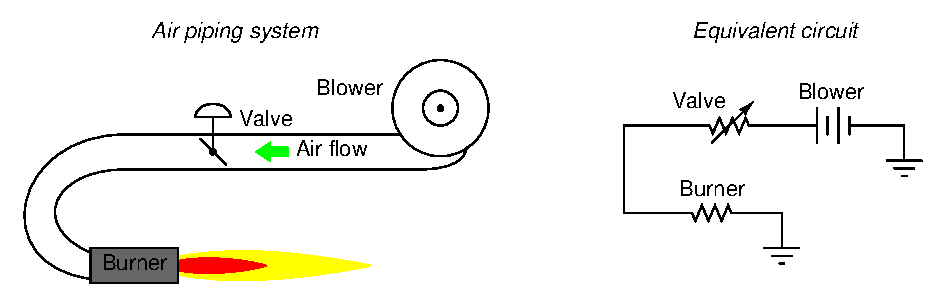
\includegraphics[width=15.5cm]{i01414x02.eps}$$

$P_1$, $P_2$ og $\Delta P$ tilsvarer henholdsvis batterispenningen, ``Brenner''-motstandens spenning og ``Ventil''-spenningen. Fra ekvivalentkretsen ser vi at ``ventilens'' spenningsfall må være trykkdifferansen mellom blåserens utløp og brennerens innløp ($\Delta P = P_1 - P_2$). Siden trykkene i denne ligningen skal angis i PSIA (absolutt trykk), må vi gjøre enhetskonverteringer for å få oppgitte trykk over i riktige enheter:

\begin{itemize}
\item{} $P_1$ = 35 "W.C.G = 1.2645 PSIG = 15.964 PSIA
\item{} $P_2$ = 8 oz./in$^{2}$ = 0.5 PSIG = 15.2 PSIA
\vskip 5pt
\item{} $\Delta P = P_1 - P_2$ = 15.964 PSIA $-$ 15.2 PSIA = 0.764 PSID
\end{itemize}

Siden gassen her er luft, kan vi bruke 1.0 for $G_g$. Temperaturen blir ganske enkelt 504.67 $^{o}$R (459.67 pluss temperatur i grader Fahrenheit).

\vskip 10pt

Til slutt er den oppgitte strømningsraten i SCFM, mens ligningen skal bruke SCFH. En enkel faktor 60 konverterer 2000 SCFM til 120000 SCFH.

\vskip 10pt

Nå er vi klare til å ``sette inn og regne'':

$$C_v = {120000 \over 963 \sqrt{{(0.764) (15.964 + 15.2)} \over {(1) (504.67)}}} = 573.53$$

\vskip 10pt

Når vi beregner rørdiameter $d$ med ligningen $C_d = {C_v \over d^2}$, ser vi at en 4.5-tommers spjeldventil vil passe svært godt i denne applikasjonen.

%INDEX% Final Control Elements, valve: sizing
%INDEX% Process: combustion furnace

%(END_NOTES)
